\documentclass[11pt,a4paper]{article}
\usepackage{lmodern}
\usepackage{float}
\usepackage{amssymb,amsmath}
\usepackage{multicol}
\usepackage{pgfgantt}
\usepackage{fontawesome}
\usepackage{ifxetex,ifluatex}
\usepackage{graphicx}
\usepackage{eso-pic}
\usepackage{wallpaper}
\usepackage{minted}
\usepackage{booktabs,makecell}
\usepackage[margin=7pt,
            font=normalsize,
            labelfont=bf,
            labelsep=space,
            position=below]{caption} % 08_03_2014
\usepackage{listings}
\usepackage{color}
 
\definecolor{codegreen}{rgb}{0,0.6,0}
\definecolor{codegray}{rgb}{0.5,0.5,0.5}
\definecolor{codepurple}{rgb}{0.58,0,0.82}
\definecolor{backcolour}{rgb}{0.95,0.95,0.92}
 \newcommand*\ruleline[1]{\par\noindent\raisebox{.8ex}{\makebox[\linewidth]{\hrulefill\hspace{1ex}\raisebox{-.8ex}{#1}\hspace{1ex}\hrulefill}}}
\lstdefinestyle{mystyle}{
    backgroundcolor=\color{backcolour},   
    commentstyle=\color{codegreen},
    keywordstyle=\color{magenta},
    numberstyle=\tiny\color{codegray},
    stringstyle=\color{codepurple},
    basicstyle=\footnotesize,
    breakatwhitespace=false,         
    breaklines=true,                 
    captionpos=b,                    
    keepspaces=true,                 
    numbers=left,                    
    numbersep=5pt,                  
    showspaces=false,                
    showstringspaces=false,
    showtabs=false,                  
    tabsize=2
}
 \usepackage{MnSymbol}
 \DeclareRobustCommand{\mysymb}{{\usefont{U}{MnSymbolC}{m}{n}\symbol{"36}}}
\lstset{style=mystyle}            
\usepackage{fixltx2e} % provides \textsubscript
\usepackage{lipsum, babel}
\ifnum 0\ifxetex 1\fi\ifluatex 1\fi=0 % if pdftex
  \usepackage[T1]{fontenc}
  \usepackage[utf8]{inputenc}
\else % if luatex or xelatex
  \ifxetex
    \usepackage{mathspec}
  \else
    \usepackage{fontspec}
  \fi
  \defaultfontfeatures{Mapping=tex-text,Scale=MatchLowercase}
  \newcommand{\euro}{€}
\fi
% use upquote if available, for straight quotes in verbatim environments
\IfFileExists{upquote.sty}{\usepackage{upquote}}{}
% use microtype if available
\IfFileExists{microtype.sty}{%
\usepackage{microtype}

\UseMicrotypeSet[protrusion]{basicmath} % disable protrusion for tt fonts
}{}
\usepackage[margin=0.787402in]{geometry}
\makeatletter
\@ifpackageloaded{hyperref}{}{%
\ifxetex
  \usepackage[setpagesize=false, % page size defined by xetex
              unicode=false, % unicode breaks when used with xetex
              xetex]{hyperref}
\else
  \usepackage[unicode=true]{hyperref}
\fi
}
\@ifpackageloaded{color}{
    \PassOptionsToPackage{usenames,dvipsnames}{color}
}{%
    \usepackage[usenames,dvipsnames]{color}
}
\makeatother
\hypersetup{breaklinks=true,
            bookmarks=true,
            pdfauthor={},
            pdftitle={},
            colorlinks=true,
            citecolor=blue,
            urlcolor=blue,
            linkcolor=magenta,
            pdfborder={0 0 0}
            }
\urlstyle{same}  % don't use monospace font for urls
\usepackage{graphicx,grffile}
\makeatletter
\def\maxwidth{\ifdim\Gin@nat@width>\linewidth\linewidth\else\Gin@nat@width\fi}
\def\maxheight{\ifdim\Gin@nat@height>\textheight\textheight\else\Gin@nat@height\fi}
\makeatother
% Scale images if necessary, so that they will not overflow the page
% margins by default, and it is still possible to overwrite the defaults
% using explicit options in \includegraphics[width, height, ...]{}
\setkeys{Gin}{width=\maxwidth,height=\maxheight,keepaspectratio}
\setlength{\parindent}{0pt}
\setlength{\parskip}{6pt plus 2pt minus 1pt}
\setlength{\emergencystretch}{3em}  % prevent overfull lines
\providecommand{\tightlist}{%
  \setlength{\itemsep}{0pt}\setlength{\parskip}{0pt}}
\setcounter{secnumdepth}{0}

\date{}

% Redefines (sub)paragraphs to behave more like sections
\ifx\paragraph\undefined\else
\let\oldparagraph\paragraph
\renewcommand{\paragraph}[1]{\oldparagraph{#1}\mbox{}}
\fi
\ifx\subparagraph\undefined\else
\let\oldsubparagraph\subparagraph
\renewcommand{\subparagraph}[1]{\oldsubparagraph{#1}\mbox{}}
\fi
\usepackage[para]{footmisc}
\usepackage{fontspec}
\usepackage{libertine}

\newcommand*{\plogo}{\fbox{$\mathcal{PL}$}} % Generic publisher logo
\ThisCenterWallPaper{1.1}{images/bg_1.jpg}
%----------------------------------------------------------------------------------------
%    TITLE PAGE
%----------------------------------------------------------------------------------------

\newcommand*{\titleGP}{\begingroup % Create the command for including the title page in the document
{\color{white}\begin{itemize}
\centering % Center all text
\vspace*{\baselineskip} % White space at the top of the page

\rule{\textwidth}{1.6pt}\vspace*{-\baselineskip}\vspace*{2pt} % Thick horizontal line
\rule{\textwidth}{0.4pt}\\[\baselineskip] % Thin horizontal line

{\LARGE Advanced Techniques in multidisciplinary Design}\\[0.2\baselineskip] % Title

\rule{\textwidth}{0.4pt}\vspace*{-\baselineskip}\vspace{3.2pt} % Thin horizontal line
\rule{\textwidth}{1.6pt}\\[\baselineskip] % Thick horizontal line

\scshape % Small caps
 \\ % Tagline(s) or further description
Optimising Orbital Profiles Of Sample Return Missions to Near-Earth Asteroids \\[\baselineskip] % Tagline(s) or further description
Wednesday, 3 \textsuperscript{th} April May 2017\par % Location and year

Edited by \\[\baselineskip]
{\Large Asheesh Sharma\par} % Editor list
\textbf{Candidate: 33074, Student: 1562159}\\
{\itshape University of Bristol \\ United Kingdom\par} % Editor affiliation
{\Large \href{https://github.com/Asheeshkrsharma/ATMD-project.git}{\faGithub} \small /Asheeshkrsharma/ATMD-project.git}
\\(includes the project code and this document in LaTeX)
\vfill % Whitespace between editor names and publisher logo

"I didn’t feel like a giant. I felt very, very small."\\
Neil Armstrong on looking back at the Earth from the Moon in July 1969.

\vspace*{2\baselineskip} % Whitespace between location/year and editors

\begin{figure}[htbp]
\centering

\resizebox{0.2\textwidth}{!}{\includegraphics{images/whitelogo.png}}


\end{figure} \\[0.3\baselineskip] % Publisher logo
{\scshape 2017} \\[0.3\baselineskip] % Year published
\par % Publisher
\end{itemize}}
\endgroup}

\begin{document}
\pagestyle{empty} % Removes page numbers
\titleGP % This command includes the title page

\newpage

\hypersetup{linkcolor=black}
\setcounter{tocdepth}{3}
\tableofcontents
\listoffigures
\clearpage

\pagestyle{plain}

\newpage
\section{Abstract}\label{motivation}
Interplanetary missions can often become fuel demanding depending on the orbital dynamics of different bodies in the solar system. This is especially true with bodies such as asteroids and comets that have a high eccentricity and inclination orbits. Missions such as sample return that involve landing on the surface of celestial objects and then returning back to Earth with samples require careful planning and optimization of different mission aspects like Earth orbit parking (from and to the Asteroid), $\Delta V$ budgets, etc.. This study investigates a systematic optimisation of orbital transits for a sample return mission from an asteroid EROS(433). In a real scenario, physical properties of such bodies are not known \footnote{except for Keplerian orbital elements through worldwide observations}. Therefore, it is required that the spacecraft rendezvous with the asteroid for sufficient time to determine its characteristics. This adds complexity to the mission planning due to the uncertainty involved with correct time windows. The objective of this study then is as follows. Given the initial (observed) conditions of an asteroid, a genetic algorithm is devised to determine the optimal choice of $\Delta V$ required for the rendezvous, insertion, sample collection and return back orbital profiles \footnote{Lambertian trajectories will be used}. The algorithm results in solutions which provide significantly improved robustness and flexibility regarding the uncertain time windows. Furthermore, the adaptiveness of the algorithm is demonstrated by applying different minimizing, maximizing, and relaxed constraints \footnote{like number of days, Energy etc.} in such missions.\\

Keywords: EROS(433), Genetic Algorithms, $\Delta V$, Sample return, Optimisation.

\ruleline{\mysymb{} }
\begin{multicols}{2}
\section{The problem statement}
The key problem is to find a globally optimum trajectories from Earth to  EROS(433) and back including the initial and final orbits around the Earth that are feasible within the capabilities of a spacecraft and the currently available launch vehicles. This analysis involves solving Lambert's problem to find the initial velocity required to travel from one point to another in a given time, initial and final position vectors. Secondly, it involves predicting the velocity when the spacecraft arrives at the destination. For a two body system, given an initial $\bar{r(t_1)}$ and final $\bar{r(t_2)}$ vector in space at different times,  the differential equation of the two body problem of the Keplerian orbit can be defined as

$$\ddot{\bar{r}}=-\mu . \frac{\hat{r}}{r^2}$$

Then the solution to the Lambert problem is the orbit for which  $\bar{r(t_1)}=\bar{r_1}$ and $\bar{r(t_2)}=\bar{r_2}$. 

For a sample return mission, the Lambert problems are two-fold. Firstly, finding velocity vectors $V_1$ and $V_2$ for low Earth orbit to EROS(433) position vectors $\bar{r(t_1)}$ and $\bar{r(t_2)}$ in a given time $\delta t_0$. Secondly, finding velocity vectors $V_3$ and $V_4$ for EROS(433) to low Earth orbit position vectors $\bar{r(t_3)}$ and $\bar{r(t_4)}$ in a given time $\delta t_1$. Although there can be perturbations due to other celestial objects in the solar system (which can sometimes be useful; gravity assists), since only a two body system is considered, everything will be calculated in the Heliocentric inertial frame (the center of the Sun). However, it is not the case when the spacecraft is in low Earth Orbit where a Geocentric inertial frame is used\footnote{same is the case for the spacecraft when it is in orbit around EROS(433)}. But simple vector mathematics can be employed there to transform the state vectors from Heliocentric to Geocentric and vice-versa. Another assumption made here is that Keplerian orbital elements of EROS(433) are known which are to be used in conjunction with Kepler's laws to calculate the position and velocity of all the objects associated with the mission profile. 
Table 1. Lists all the orbital elements acquired from JPL's Horizon database.

The focus of this analysis is not on the various solution of Lambert’s problem, but the application of it for interplanetary mission design. Therefore, for this analysis, an open source MATLAB code is used for the solution to Lambert’s problem. It is also worth noting some interesting characteristics of the EROS(433) asteroid. Although the asteroid has a minor inclination of only 1.7 degrees off of the ecliptic plane, the really large Semi-major axis results in a highly inclined orbit. Therefore, there will be no solutions found with only directly tangential burns if time-frame of fewer than 365 days is considered in the search space. The EROS asteroid also has a much larger eccentricity than the orbit of Earth. However, it can be seen from the table 1. that the asteroid actually comes within the orbit of Earth. Finally, there is a large difference between Longitude of Ascending node and the argument of perigee of Earth and EROS(433), which means that departing from earth would require a lot of energy than compared to arriving from EROS(433).

\end{multicols}
\begin{table}[H]
\label{tab:mytable}
\centering
\caption{Keplerian orbital elements}
\begin{tabular}{c*{4}{r}}
\specialrule{1pt}{0pt}{0pt}
    Element                            & Symbol    & Earth                  & EROS(433)\\
    \hline\addlinespace
    Semi-major axis [Km]               & $a$       & 149598023              & 2.18096$\times 10^8$\\
    Eccentricity                       & $e$       & 0.01629                & 0.22254435\\
    Longitude of Ascending Node (deg)  & $\Omega$  & 348.73936              & 3.043259456\\
    Argument of perigee (deg)          & $\omega$  & 114.20783              & 1.7881167\\
    True anomaly (deg)                 & $\mu$     & 1.108533               & 3.575782\\
    Inclination (deg)                  & $i$       & 0.002961               & 1.0827850\\
    Mean motion (deg/sec)              & $M$       & 1.99097$\times 10^-7$  & 1.1310488 $\times 10^-7$\\
    \bottomrule
\end{tabular}%
\end{table}
\ruleline{\mysymb{} }
\begin{multicols}{2}
\section{Mathematical model}
\begin{figure}[H]
\centering
\includegraphics{images/model.pdf}
\caption{The mathematical model and calculations}
\end{figure}
Figure 1 shows the mathematical model of the considered problem. It involves three basic phases.

{\LARGE{{\fontspec[Ligatures=Discretionary]{Junicode}<1>}}} From the Keplerian orbital elements obtained from the JPL HORIZON database (table 1), current (since EPOCH) heliocentric cartesian state vectors (position $r$ and velocity $v$) are calculated. First, the state vectors in the perifocal frame are calculated.

$r_p = (\frac{h^2}{\nu}) \times (\frac{1}{1 + e\times cos(\mu))} \times (cos(\mu)\times\begin{bmatrix}1\\0\\0 \end{bmatrix} + sin(\mu)\times\begin{bmatrix}0\\1\\0 \end{bmatrix})$

$v_p = \frac{\nu}{h}\times(-sin(\mu)\times\begin{bmatrix}1\\0\\0 \end{bmatrix} + (e + cos(\mu))\times\begin{bmatrix}0\\1\\0 \end{bmatrix})$
$\text{where } h=\sqrt{\nu\times a\times(1-e^2)} \text{ and } \\ \nu \text{ is the gravitantional constant of the \\\major governing body}$

Then, the perifocal vectors are converted to Cartesian by multiplying them with a rotational matrix $Q_px$\footnote{which depend on the type of convetion is used. Such as ECI, GEO etc.. This is given in the Appendix}. After obtaining $r_1$ and $r_2$ helio centic positions vectors of the spacecraft and EROS(433) respectively, required lambetian velocities, $v_1$ and $v_2$ in a given time $\delta t_0$ can be determined using the lambert solution. Using the calculated $r_1$, $r_2$, $v_1$ and $v_2$, orbital elements ($\mu_1$, $\mu_2$) of LEO to EROS(433) are calculated. 
\\
\\
{\LARGE{{\fontspec[Ligatures=Discretionary]{Junicode}<2>}}} Now that the space craft has reached EROS(433), it needs some time $\delta t_1$ to collect samples, gather scientific data and determine its physical characteristics \footnote{$\delta t_1$ also includes the time spent in return orbital maneuvers}. Therefore, the new position vectors are to be calculated for the spacecraft ($r_3$) (which took $\delta t_1$ amount of time at EROS) and Earth $r_4$ (which took $\delta t_0+\delta t_1$). This is essentially the inverse process of {\LARGE{{\fontspec[Ligatures=Discretionary]{Junicode}<1>}}}. Using the calculated $r_3$, $r_4$, $v_3$ and $v_4$, orbital elements ($\mu_3$, $\mu_4$) of EROS(433) to LEO are calculated. 
\\
\\
{\LARGE{{\fontspec[Ligatures=Discretionary]{Junicode}<3>}}} Two key measures are calculated to ultimatly detremine the effciency and robustness of the entire mission profile. Firstly the characteristic velocity (also know as hyperbolic excess velocity) |$\Delta V$| is the overall change in velocity. This can be calculated as

$$|\Delta V|=|v2-v1|+|v4-v3|$$


Secondly, the characteristic energy ($C_3$) necessary to leave Earth and start on the transfer orbit and vice versa is a key measure to evaluate the amount of excess specific energy per mass required to complete the maneuvers. This can be calculated as

$$C_3=|v2-v1|^2+|v4-v3|^2$$

Because the solution to Lambert’s problem is dependent on the time of flight as well as the position, different solutions can be obtained for the same launch time from Earth for different arrival times at Eros. The opposite is true as well, varying launch date and keeping the same arrival time will also change the solution to Lambert’s problem. Therefore, there are two independent variables to analyze when finding a solution to Lambert’s problem. Therefore, the times $\delta t_0$ and $\delta t_1$ are crucial parameters for the optimization problem. Furthermore, the low earth orbital parameters, especially the semi-major axis and inclination also effects |$\Delta V$|. In the next section, this optimization problem is mathematically formalized.
\end{multicols}
\ruleline{\mysymb{} }
\begin{multicols}{2}
\section{Optimisation}\label{motivation}
\end{multicols}

\begin{figure}[H]
\centering
\includegraphics[width=\textwidth-85pt]{images/optimisation.pdf}
\caption{Optimisation problem}
\end{figure}

\begin{multicols}{2}
\subsection{Decision Variable: Transit times}
Figure 2 shows the formalized $\Delta V$ minimization problem where all the decision variables are constrained with compound inequalities. Based on the discussion in the previous section, $\delta t_0$ and $\delta t_1$ are time limits in which the spacecraft has to travel from and to Earth respectively \footnote{The limits were found based on the ephemerides mentioned in the table}. It can be observed that $\delta t_0$ and $\delta t_1$ are the only constraints which directly affect $v_1$, $v_2$, $v_3$ and $v_4$ calculations for the transit orbits. This is to increases robustness when the spacecraft arrives at EROS(433)  for possible rendezvous in order to determine the Asteroid's physical characteristics before orbit insertion \footnote{although physical characteristics of EROS(433) is known in the problem, they were not known when the actual mission (NEAR-Shoemaker) was executed}. However, when the lambert problem is solved, a retrograde orbit is chosen (an external constraint)  always. This means that the resulting orbits will always be shorter in distance but might have a slightly higher |$\Delta V$|. Secondly, the optimization does not consider $C_3$ at it exponentially decreases with |$\Delta V$| automatically.

\subsection{Decision Variable: Orbital}
Since all the the rest of constraints ($i_2$, $i_2$, $r_{leo1}$, $r_{leo2}$, $\mu_{leo1}$, $\mu_{leo2}$) determine the characteristics of low earth orbits, they always remain active during the optimisation. Figure 3 shows the keplerian elements which are used to determine the position of a celestial body moving in an orbit around a bigger body.
\begin{figure}[H]
\centering
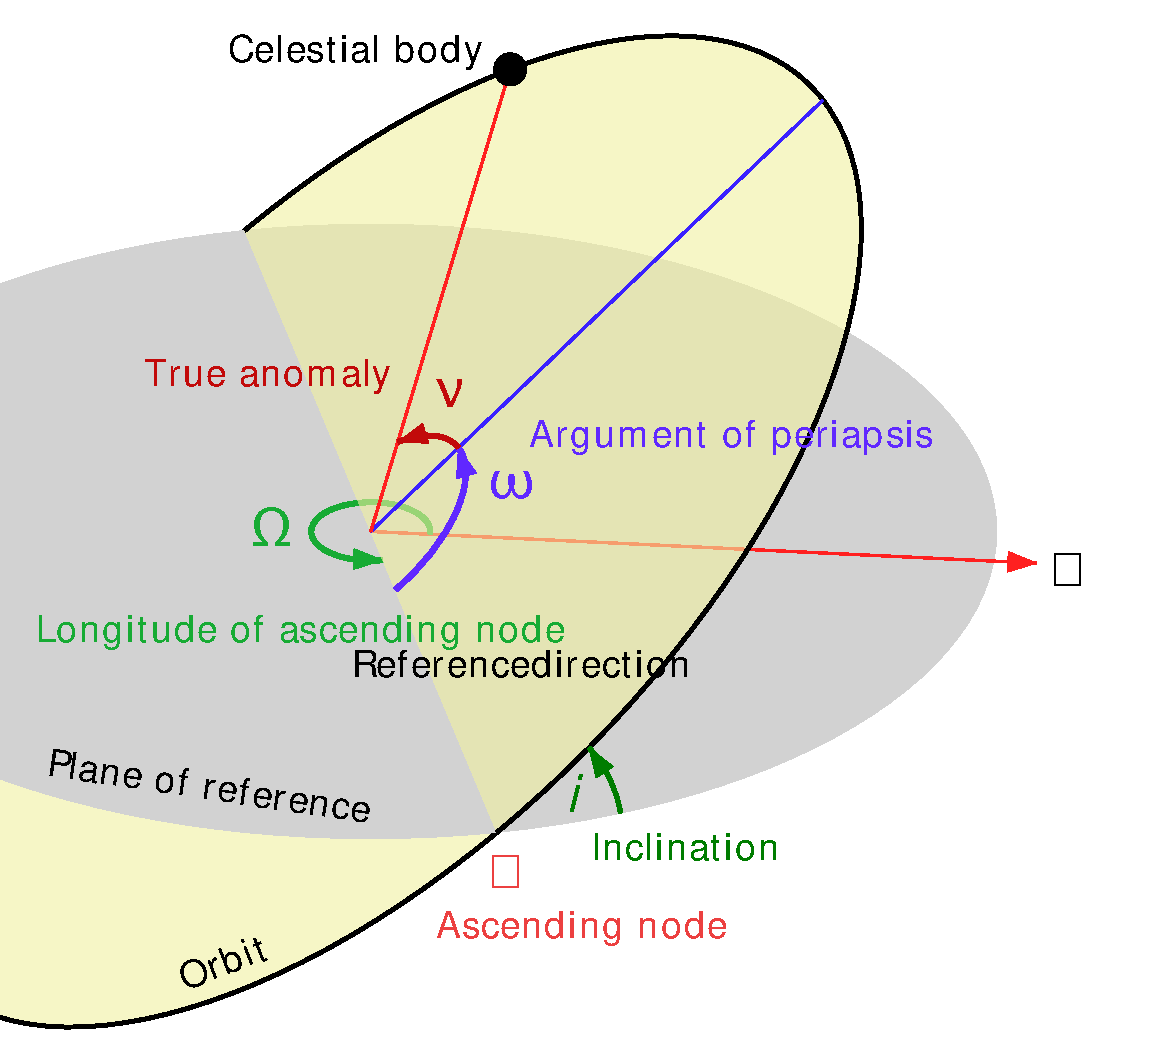
\includegraphics[width=3.5in]{images/orbital.pdf}
\caption{Keplerian orbital elements}
\end{figure}
Let's assume a two-body system in which a small body is orbiting a much bigger one. The plane of reference (figure 3; pale blue) is defined as the plane which does not change inertially for the bigger body. The angle which the smaller body makes with the plane of reference in the vertically-orthogonal direction is called the inclination $i$. A plane which then makes the same angle $i$ with the plane of reference is called the orbital plane (figure 3; pale yellow) in which the smaller body moves. In the orbital plane, the angle made by the smaller body with the horizontal axis (blue line in the pale yellow plane) is called the true anomaly ($\mu$).

For the optimization, the effect of true anomaly and inclination are twofold. If the inclination is significantly large (which is the case here), a spacecraft traveling to the orbiting body will have to apply 'out of plane' burns which will inherently increase the |$\Delta V$| significantly. Secondly, the true anomaly of the orbiting body will determine the number of in-plane small adjustment burns required for maintaining the transit orbit. Since only circular orbits are considered, the semi-major and semi-minor axis become equal to $r_{leo\{1,2\}}$ for LEO-1 and LEO-2 during the transits. As the inclination and the true anomaly of EROS(433) at epoch were very high, $r_{leo\{1,2\}}$ constraints will intuitively distribute the adjustments burns evenly over the orbital plane. 
\end{multicols}
\ruleline{\mysymb{} }
\begin{multicols}{2}
\section{Optimiser}

From the mathematical model, it becomes clear that the problem can not be solved with integer programming because of the precision required which lies in the real space. Furthermore, such missions can have very different outlines depending on the kind of maneuvers chosen. For example, if the spacecraft is to be accelerated using Earth's orbit, then the keplerian model has to replaced with the Hohman's gravity assist model as it requires burns in between the initial and final positions. Secondly, the formulation of characteristic velocity (termed $\Delta VEGA$\footnote{Earth Gravity Assist}) will be different. Since there are a plethora of ways to design the missions, the entire profile is not expressible in a single function. Therefore, optimization methods which involve finding the steepest "direction" can be really difficult to implement. It can also be noted that even if it was possible, gradient-based methods can get stuck in a local minimum and their performance is dependent on initial values of design variables. Therefore, an optimizer is required which allows changing the decision variables, does not require the calculation of gradient so that modeling can remain descriptive\footnote{ideally should work like mathematical plugins; simply replace one with other} and converges globally. Thus, methods like particle swarm and genetic algorithm are favorable.

\section{Genetic algorithm and components}


The figure 5 shows the implemented genetic algorithm which has following major components.

\subsection{Chromosomes}
The first process encountered in the GA is generating a set of initial solutions which can be randomly generated or specified using other methods. A chromosome contains genes which are manipulated every time in the algorithm. Therefore a careful design choice has to be made so that the solutions remain valid and constrained. For this optimization, a floating number based coding scheme was developed as shown in figure 4.

\begin{figure}[H]
\centering
\includegraphics{images/chromosome.pdf}
\caption{Chromosome}
\end{figure}

Each gene represents the constraints being applied to the optimization problem as mentioned in figure 2. When the population is initialized all the genes are randomly generated to lie within their respective ranges.

\begin{figure}[H]
\centering
\includegraphics[width=2.5in]{images/GA.pdf}
\caption{The genetic algorithm}
\end{figure}

\subsection{Evaluation}
After generating an initial population of chromosomes, they are evaluated by invoking the model subroutine which calculates the |$\Delta V$| profile. The convergence results and efficiency of genetic algorithm heavily relies on the responsiveness of the fitness function. Initially, the fitness function is simply $f|=\Delta V|$ where a lower score means higher fitness. The fitness function will be further improved in the rest of the sections as further investigation is made. 



\subsection{Selection, Crossover and mutation}
Elitism is preferred over iterations while taking a special care of diversity. Only a fixed percentage (out of the total number of chromosomes) of fittest chromosomes are randomly crossed over. If the children are worse than parents, they will be chosen using the simulated annealing coin-flip strategy.  For instance, let's say a child is worse than any or both of parents, probability of accepting the worse child is calculated as 
$$P=e-(f_c-f_p)/T$$

where, $T= T_0\timese^{-ak}$. This ensures that a balance is maintained between elitism and diversity. The annealing process is reduced as the number of iterations k increases. The crossover operator (Shown in figure 6) works by randomly choosing a crossover point $x$ which can lie between one and 7. Then, the genes from blue and green chromosomes are combined as shown in the figure. 

\begin{figure}[H]
\centering
\includegraphics{images/OnePointCrossover.pdf}
\caption{Single point corssover}
\end{figure}

Special care is taken to select the crossover point by slightly biasing it to the dominating parent. Let's assume that the blue gene was superior to green, and $x=4$. Choosing  $x=4$ will mean that the child will have more genes from green (which is inferior). In that case, $x$ will be biased simply as $x=7-x$.

After crossing over, the children are then merged with the rest of the population. Then, the mutation phase begins where every gene in a chromosome will be mutated based on a fixed probability $p_m$ which is chosen to be 0.45 empirically. For every gene, if a randomly generated number is bigger than $p_m$, then a slight increase or decrease is made which such that the resultant still lies within the ranges mentioned in previous section (figure). 

\subsection{Convergence}
The GA is terminated if no improvement is made for a significant number of iterations or when it reaches the maximum number of iterations.
\end{multicols}


\begin{multicols}{2}
\section{Results}\label{motivation}
\end{multicols}

\begin{figure}[H]
\centering
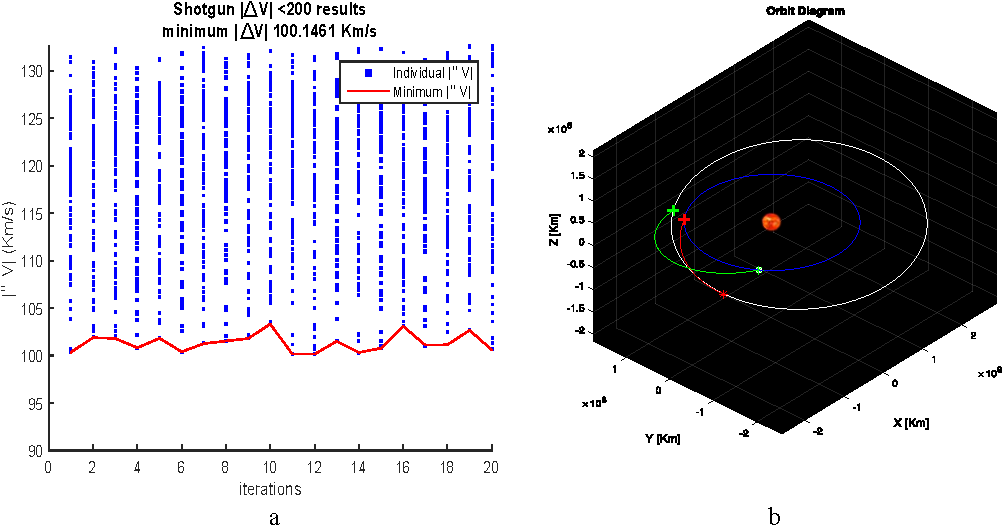
\includegraphics[height=3.5in]{images/shotgun.pdf}
\caption{Minimum |$\Delta V$| observed during shotgun iterations}
\end{figure}
\begin{multicols}{2}
\subsection{Results from shotgun}
Since there were no reference convergence results available for the given problem \footnote{This is a hypothetical mission, therefore there was no solution available. Secondly, an exhaustive search was avoided because it took "too long" to end}, shotgun results were used as a baseline for optimization. 200 iterations of 100 random solutions were generated and the best solution was found based on the lowest |$\Delta V$| as shown in Figure 7a. It is evident that since there is no method to improve solutions over iterations, individual solutions at every respective iteration are heavily spread. The resultant orbital diagram is shown in figure (). The round trip journey takes 292 days, with a total |$\Delta V$| of  100.146 $Km/s$. The suggested initial Low earth orbit has an altitude of $3,891 Km$ with a true anomaly of $204^o$ and an inclination of $0^o$. For the return journey (about 198 days later), the return low earth orbit has an altitude of $1,447$ $Km$ with a true anomaly and inclination of $12^o$ and $3^o$ respectively. There are following key observations:

1. Although overall |$\Delta V$| budget is feasible, the required $C_3$ for the transits from Low Earth orbit and back is really high. Therefore, $C_3$ should be a secondary fitness criterion.

2. The constraints on inclinations for the arrival and departure low earth orbits can be relaxed since changing them does not affect the results much\footnote{a standard deviation of $90^o$ was applied in the shotgun for arriving and departing LEO inclinations. This resulted in a minor change of $\pm 12.319 Km/s$ in the $\Delta V$}. All other constraints were kept constant.

3. There is also some consideration required on the allowable scatter of the solutions in every iteration. A method has to be developed which allows the scattering to reduce over iterations in a consistent manner. At the same time, the method should be able to maintain the diversity of solutions so that final iteration has similar $\Delta V$ budgets but with a potentially different total journey time and $C_3$.

From the above discussion, it can be seen that a genetic algorithm can be a really good optimizer. For instance, Monte-Carlo methods can be used efficiently to minimize |$\Delta V$| as well but it will be harder to come up with equivalently similar solutions which have different orbital parameters. Secondly, it is always easier to switch between different fitness functions to suit different optimization objectives. Keeping the above goals in mind, a new fitness function was formulated as shown below.

$$\\f=W_1\times|\Delta V| + W_2\times S$$
where
$$S= \frac{|\Delta V_{max}| - |\Delta V_{min}|}{|\Delta V_{min}|}$$
\end{multicols}

\begin{figure}[H]
\centering
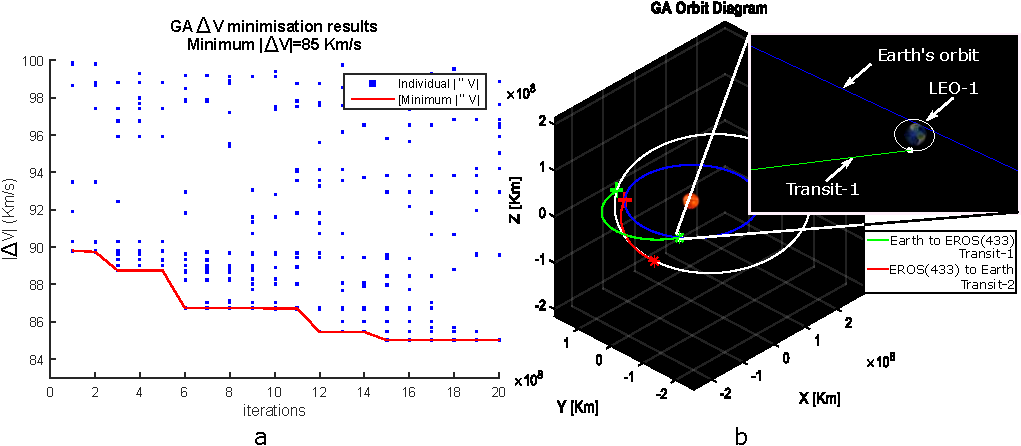
\includegraphics[]{images/Genetic.pdf}
\caption{Minimum |$\Delta V$| observed using GA}
\end{figure}

\begin{multicols}{2}

The new fitness $f$ is a function of weights $W_1$ and $W_2$ of $\Delta V$ and Scatter $S$ in the population respectively. These weights are dynamically changed in every iteration. $W_2$ increases in every iteration, whereas $W_1$ decreases. This ensures that the spread is reduced effectively. Another aspect of introducing $S$ into the fitness equation is that it becomes easier to test for convergence. That is, if the deviation in $S$ has become negligible over some of the past iterations, it can be assumed that the optimization has converged.

\subsection{Results from a Genetic Algorithms}

A result of optimization, the minimum $\Delta V$ was found to be 85 $km/s$ (figure 8a) which is a significant improvement over the result from the shotgun. For both low earth orbits, the inclination was also minimized to $i_{leo1}=3^0$ and $i_{leo2}=0^o$ (can be visibly seen in figure (8b)), which makes sense as the optimization tried to avoid out of plane burns. The true anomalies for the departing and arriving LEOs were $\mu_{leo1}=91^o$ and $\mu_{leo2}=98^o$ which are very nominal. $r_{leo1}$ and $r_{leo2}$ were found to be 3,698 $km$ and 1,447 $km$ respectively. Following are the key observations:

\subsection{Efficiency of the determined trajectories.}
On the return trajectory the closest approach to Earth ($r_{leo2}$ = 1,243 $km$) lies within the noticeable atmosphere of the Earth and hence the drag will draw the spacecraft into a ballistic reentry. But since the spacecraft will approach at relatively low inclination $i_{leo2}=2^o$, very small amount of $\Delta V$ will be required for correction. Therefore this is ignorable. It is also assumed that the launch vehicle is capable of placing the spacecraft in a parking orbit LEO1. It is estimated that 10 km/s of $\Delta V$ is required to boost to LEO1. Finally, to boost from LEO1 to the transit trajectory requires a total of 54.2 $km$ of $\Delta V$. Since the inclinations are low, the $\Delta V$ gained from launch vehicle can be harness and the rest of the requirement can be met through gravitational slingshots around Earth. 

\subsection{Efficiency of the spread fitness function}

In figure 8a, it is evident that the optimization process attempts to center and tighten the scatter of $\Delta V$. This has two primary effects. Firstly, the chromosomes become more centered and separated into similar solution (in the last iterations, most of the solutions have converged to the actual solution). Secondly, the weights for $\Delta V$ and $S$ in $f=W_1\times\Delta V+\W_2\times\S$ efficiently balances diversity and elitism. However, this comes at some expense of increased $\Delta V$. The optimization is be hindered greatly if the S is not linearly related to the $\Delta V$. Therefore, a possible remedy would be to empirically determine the true values of $W_1$ and $W_2$.

\subsection{Changing the objective function}
The optimal transfer orbits are very dependent on the type of mission and are not necessarily a minimum value. This analysis was done on interplanetary transfers where the spacecraft intended to orbit the asteroid upon arrival, land and then come back to Earth. However, different types of missions would have different requirements on them. For example, a mission to impact the asteroid would not depend as much on \end{multicols}

\begin{table}[H]
\label{tab:mytable}
\centering
\caption{Optimising with different objectives}
\begin{tabular}{c*{5}{r}}
\specialrule{1pt}{0pt}{0pt}
    DVs            & Shotgun           & GA $\Delta V$       & GA $\delta t_{0}+\delta t_{1}$  & GA $C_3$\\
    \hline\addlinespace
    $\delta t_0$   & 198               & 218                 & 167                             & 248\\
    $\delta t_1$   & 94                & 94                  & 19                              & 10\\
    $\mu_{leo1}$   & 204               & 91                  & 341                             & 354\\
    $\mu_{leo2}$   & 12                & 98                  & 52                              & 230\\
    $i_{leo1}$     & 0                 & 3                   & 3                               & 3\\
    $i_{leo2}$     & 3                 & 2                   & 2                               & 2\\
    $r_{leo1}$     & 3,891             & 3,698               & 3,082                           & 3,143\\
    $r_{leo2}$     & 1,447             & 1,243               & 6,712                           & 3,631\\
    \specialrule{1pt}{0pt}{0pt}\\
    $\Delta V$     & 100.09192         & 85.34               & 88.42                           & 90.174\\
    $C_3$          & 3.84$\times 10^3$ & 2.912$\times 10^3$  & 3.97 $\times 10^-3$           & 3.212 $\times 10^3$\\
    \bottomrule
\end{tabular}%
\end{table}



\begin{multicols}{2}
the incoming velocity (which is evident from the table below). Therefore, it would be more advantageous to minimize the characteristic energy of this transfer. Another thing to consider is a human mission to the EROS(433) asteroid. If this were the case, it would most likely be advantageous to minimize the transfer time between Earth and the asteroid. Therefore, different types of objective functions were also optimized as shown in table 2.


\section{Conclusion}
This study has presented a method to determine a robust $\Delta V$ minimisation framework using genetic algorithms. It was found that the genetic algorithm based optimization is a great choice of optimiser for solving the problem. However, since the studied problem didn't have an already known global optimum (through other methods), global optimality of the algorithm can not be determined.

\section{Future work}

The scope of this analysis is a basic application of Lambert’s problem. These trajectories are purely ballistic transfer trajectories. In reality, spacecraft will typically perform maneuvers during the transfer. Because of this, there are more trajectories available than the simple ballistic trajectories. However, the range of launch windows gives a very good idea for mission planning of transfer trajectories. Also beyond the scope of this analysis is the possibility of using gravity assists and Hohmann transfers for an ideal transfer. Thus using the framework discussed in the study, such mathematical models can be implemented with ease. However, to find a globally optimal solution, in that case, these models should not be tested individually, but as a hybrid mutation method. Secondly, although global optimality is not guaranteed, Monte-Carlo methods can also be used as a mutation to further improve the solution given by the internal components of the GA. This analysis is also limited in its accuracy. The analysis assumes that the orbit of Earth and EROS are perfectly Keplerian. Secondly, it is also assumed that both the objects have zero deviations in their gravity. Therefore, including perturbations should also be considered. Thirdly, it is assumed that spacecraft is already in orbit, therefore, the launch vehicle trajectories and its addition to the $\Delta V$ is not considered.

\end{multicols}

\end{document}